%!TEX root = /Users/jakubkonka/Thesis/Thesis.tex
\chapter{Digital Marketplace} % (fold)
\label{cha:dmp}

\section{Principles of Operation} % (fold)
\label{sec:principles_of_operation_dmp}
The Digital Marketplace (DMP) is a market-based framework for trading wireless communications services. In its simplest form, there are three main groups of actors involved in the operation of the DMP: \emph{subscribers}, \emph{network operators}, and \emph{market provider}. The subscribers are the end-users of the communications services, and they act as the buyers in the DMP. The network operators, on the other hand, act as the sellers/bidders. Lastly, the market provider is tasked with operating the DMP; thus providing common platform for all actors involved. It is left open-ended who should be the market provider; however, one of the following three choices is the most likely: a regulatory body, a consortium of network operators, or a single network operator on behalf of the regulatory body \cite{DMIrvine02}.

\begin{figure}[t]
	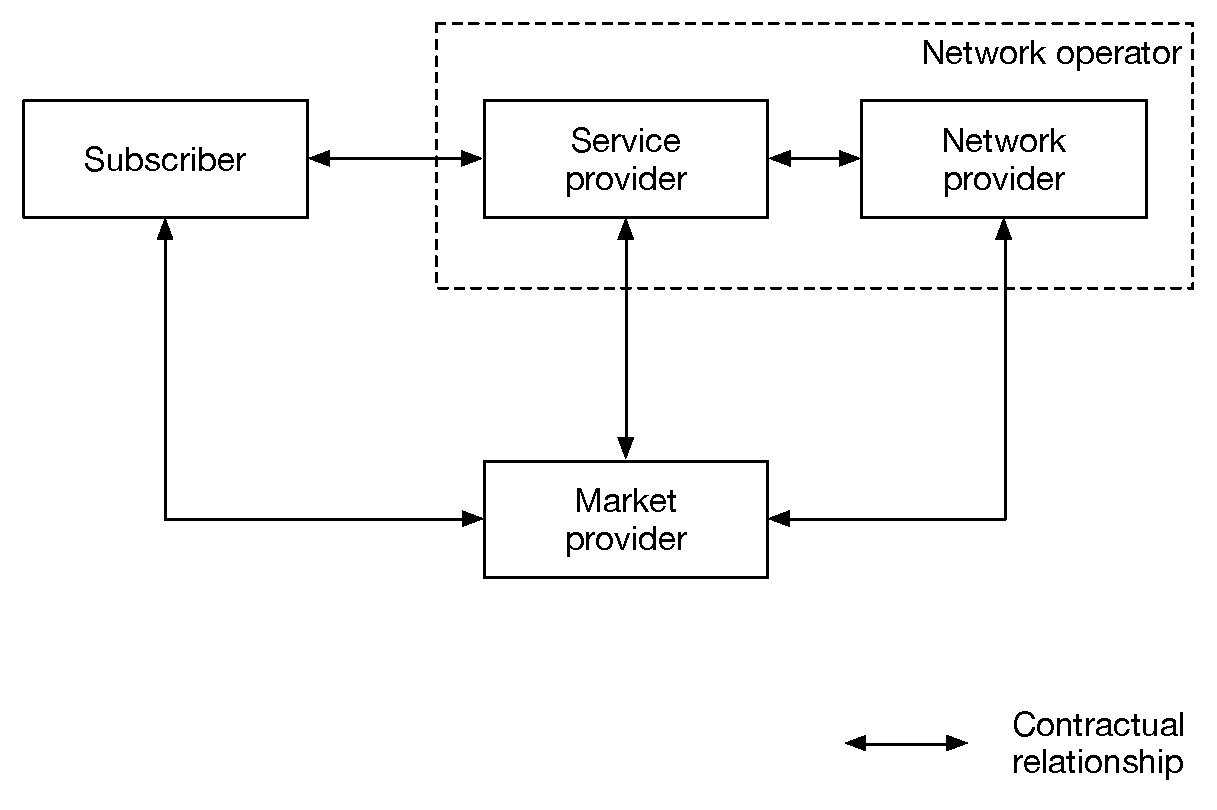
\includegraphics[width=\figsize]{DMP/Figures/dmp_model}
	\caption{The business model of Digital Marketplace (adapted from~\cite{DMIrvine02})}
	\label{fig:dmp_model_dmp}
\end{figure}
% section principles_of_operation_dmp (end)

\section{Network Selection Mechanism} % (fold)
\label{sec:network_selection_mechanism_dmp}
The process of negotiation (or the network selection mechanism) in the DMP is based on a procurement first-price sealed-bid auction. Unlike in a standard procurement first-price sealed-bid auction, the winning bid is a weighted (convex) combination of both the network operator's monetary bid and their reputation rating; we will refer to it as the \emph{compound bid}. The network operator is elected as the winner of the auction if their compound bid is the lowest in value, and accrues their monetary bid minus the cost of supporting the service. The monetary bid is equivalent to the price of supporting the service by the network operator. The precise definition of the price is left open-ended; one possibility, for example, would be to charge the buyer per unit of bandwidth. The weights in the compound bid are set by the subscriber before each auction, and are announced to the network operators. This effectively gives the subscriber the freedom to choose any combination ranging from: a low price for the service but also poor quality; to a high quality but for a high price \cite{DMLeBodic00}.

Since the communications services are traded on an individual service level, it might be difficult for the subscriber to judge the overall quality of the services supplied by a particular network operator \cite{DMIrvine02}. Therefore, one of the fundamental assumptions governing the operation of the DMP is that, by registering in the DMP, network operators agree to report on their contract fulfillments to the market provider; that is, they agree to report a binary value denoting the success in delivering the service to the subscriber within the agreed Quality of Service (QoS) bounds \cite{DMLeBodic00}. The value of $0$ denotes a failure, while the value of $1$ a success. The latest $d$ ($d>1$) reports are then used to compute the reputation rating of the network operator which will be used when a new service request arrives in the marketplace. Hence, assuming network operator $i$ admitted $t$ service requests, the formula for computing a reputation rating update is as follows (cf.~Section~3.2 in~\cite{DMLeBodic00})
\begin{equation}
    \label{eq:reputation_rating_update_dmp}
    r_i^{t+1} = \sum_{k = t-d}^d \frac{1 - report_i^k}{d},
\end{equation}
where $report_i^k$ denotes the $k^{\text{th}}$ binary report of the network operator $i$. Note that Equation~\eqref{eq:reputation_rating_update_dmp} implies $r_i^{t+1} = 0$ if the network operator $i$ has successfully delivered $d$ services to the subscriber, while $r_i^{t+1} = 1$ if has failed in all $d$ attempts. Furthermore, Equation~\eqref{eq:reputation_rating_update_dmp} implies that if the operator is consistently unreliable, their performance is reflected accordingly by their reputation rating history. Whilst, similarly, one failure in delivering the service does not immediately render a network operator unreliable; rather, it marginally affects their updated reputation rating. At the same time, at the end of each contract, the subscriber may report on their satisfaction (or Quality of Experience, QoE) with the service, for example, by submitting a mean opinion score in case of real-time services, and achieved throughput for non-real-time ones. The reputation rating update formula in Equation~\eqref{eq:reputation_rating_update_dmp} could then be modified to incorporate QoE, for instance, by taking an appriopriately weighted composition of both network operator's and subscriber's reports. Since this paper just barely scratches the surface of the reputation rating system maintained by the DMP, and the concept of QoE, the Readers are referred to \cite{DMLeBodic00, LeBodicThesis, DMIrvine02, DMMathur02, DMIrvine01, DMMcDiarmid06} for a more in-depth treatment of the former and to~\cite{Kilkki2008, BrooksHestnes2010, Fiedler2010, Shaikh2010} of the latter.
% section network_selection_mechanism_dmp (end)

\section{Contributions of This Research to Digital Marketplace} % (fold)
\label{sec:contributions_of_this_research_to_digital_marketplace_dmp}

% section contributions_of_this_research_to_digital_marketplace_dmp (end)

\section{Summary} % (fold)
\label{sec:summary_dmp}

% section summary_dmp (end)
% chapter digital_marketplace_dmp (end)